!TeX root = ../ejemplo.tex
\section{Tecnologías de Identificación y Control de Acceso}
\subsection{Códigos QR}

Actualmente, las credenciales del Instituto Politécnico Nacional (IPN) incluyen un código QR que, al ser escaneado, proporciona acceso a la información del estudiante. Este código QR contiene datos esenciales como el nombre completo, número de boleta, carrera en la que está inscrito y su fotografía. Además, en algunas unidades académicas del IPN, los códigos QR se utilizan como medio de verificación de identidad para el ingreso a las instalaciones mediante torniquetes electrónicos.

En la elaboración de nuestro trabajo terminal, el código QR desempeña un papel fundamental en la corroboración de la identidad de los estudiantes. Dado que las credenciales escolares contienen un código QR, se puede aprovechar su capacidad para almacenar y transmitir información de manera segura y rápida. Este enfoque permite verificar los datos del estudiante mediante un escaneo simple, reduciendo el tiempo necesario para validar su identidad. Al escanear el código QR de la credencial, el sistema accede a los datos del alumno, lo cual facilita confirmar si coinciden con la persona que se presenta al Examen a Título de Suficiencia (ETS).

Un código QR es un tipo de código de barras bidimensional que puede ser leído por teléfonos inteligentes o dispositivos especializados en su lectura. Al escanear un código QR, los dispositivos pueden acceder directamente a mensajes de texto, correos electrónicos, sitios web, números de teléfono, entre otros \cite{CitaA01}.

\subsubsection{Anatomía y funcionamiento}

A continuación, se describen los principales componentes estructurales de un código QR:

\paragraph{Patrones de detección de posición}

\begin{figure}[htbp]
	\begin{center}
		\fbox{
\includegraphics[width=.24\textwidth]{images/img01}}
		\caption{Patrones de detección de posición \cite{CitaA01}.}
		\label{fig:PatronesDeDeteccion}
	\end{center}
\end{figure}

Estos patrones se encuentran en tres de las esquinas del código QR. Gracias a ellos, el escáner puede reconocer y leer el código rápidamente, ya que indican la orientación del mismo y facilitan su detección.

\paragraph{Patrones de alineación}

\begin{figure}[htbp]
	\begin{center}
		\fbox{
\includegraphics[width=.24\textwidth]{images/img02}}
		\caption{Patrones de alineación \cite{CitaA01}.}
		\label{fig:PatronesAlineacion}
	\end{center}
\end{figure}

Estos patrones permiten corregir distorsiones cuando el código QR se imprime sobre superficies curvas. Su tamaño y cantidad varían dependiendo de la cantidad de información almacenada.

\paragraph{Patrones de temporización}

\begin{figure}[htbp]
	\begin{center}
		\fbox{
\includegraphics[width=.24\textwidth]{images/img03}}
		\caption{Patrones de temporización \cite{CitaA01}.}
		\label{fig:Temporizacion}
	\end{center}
\end{figure}

La alternancia de módulos negros y blancos determina el sistema de información, también conocido como cuadrícula de datos. Estas líneas permiten al escáner identificar la estructura del código.

\paragraph{Información sobre la versión}

\begin{figure}[htbp]
	\begin{center}
		\fbox{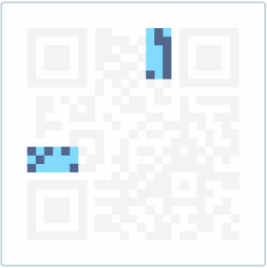
\includegraphics[width=.24\textwidth]{images/img04}}
		\caption{Información sobre la versión \cite{CitaA01}.}
		\label{fig:Version}
	\end{center}
\end{figure}

Estos marcadores indican cuál de las 40 versiones del código QR se está utilizando. Generalmente, las versiones utilizadas van de la 1 a la 7.

\paragraph{Información del formato}

\begin{figure}[htbp]
	\begin{center}
		\fbox{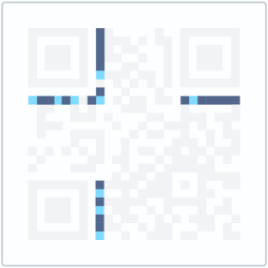
\includegraphics[width=.24\textwidth]{images/img05}}
		\caption{Información del formato \cite{CitaA01}.}
		\label{fig:Formato}
	\end{center}
\end{figure}

Este componente contiene datos sobre la tolerancia a errores y el patrón de enmascaramiento. Su función es facilitar el proceso de escaneo.

\paragraph{Código de corrección de datos y errores}

\begin{figure}[htbp]
	\begin{center}
		\fbox{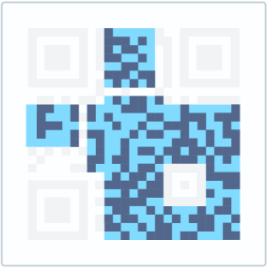
\includegraphics[width=.24\textwidth]{images/img06}}
		\caption{Código de corrección de datos y errores \cite{CitaA01}.}
		\label{fig:CorreccionErrores}
	\end{center}
\end{figure}

El sistema de corrección de errores comparte espacio con los datos almacenados. Esto permite recuperar información incluso si una parte del código está dañada o ilegible \cite{CitaA01}.

\paragraph{Márgenes}

\begin{figure}[htbp]
	\begin{center}
		\fbox{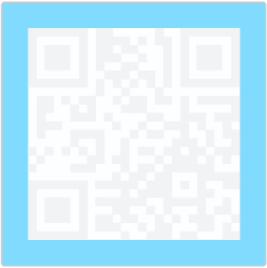
\includegraphics[width=.24\textwidth]{images/img07}}
		\caption{Márgenes o zonas quietas \cite{CitaA01}.}
		\label{fig:Margenes}
	\end{center}
\end{figure}

Los márgenes o zonas quietas rodean el código QR y permiten que el lector distinga claramente sus límites. Son fundamentales para que el escáner identifique correctamente el código.

\subsubsection{Fiabilidad y aplicaciones en seguridad}

Los códigos QR están diseñados para mantener su legibilidad incluso si están parcialmente dañados u oscurecidos. Esto es posible gracias a su capacidad de corrección de errores, que inserta la información varias veces en el patrón del código. Dependiendo del nivel de seguridad utilizado, un código QR puede seguir siendo legible incluso si se ha perdido hasta un tercio de su información original.

Esta característica los convierte en una herramienta muy confiable para almacenar datos, especialmente en aplicaciones donde la seguridad y la verificación rápida de identidad son críticas. Por ello, su uso en credenciales escolares representa una solución eficaz para garantizar el acceso controlado a instalaciones o servicios institucionales.